%!TEX root = da2020-10.tex

\Chapter{10}{Sinkless Orientation}

\noindent
In this chapter we will study the complexity of \emph{sinkless orientation}, a problem that was introduced in the previous chapter. This is a problem that is understood well: we will design algorithms and show that these are asymptotically optimal.

Recall that sinkless orientation is the problem of orienting the edges of the tree so that each internal node has got at least one outgoing edge. We begin by studying sinkless orientation on paths (or $(2,2)$-biregular trees), and show that we can easily argue about local neighborhoods to prove a tight lower bound result. However, when we switch to $(3,3)$-biregular trees, we will need the round elimination technique to do the same.

\section{Sinkless Orientation on Paths} \label{sec:so-paths}

We define \emph{sinkless orientation on paths} to be the following bipartite locally verifiable problem $\Pi = (\Sigma, \collA, \collP)$. The alphabet is $\Sigma = \{ \mI, \mO \}$, with the interpretation that $\mI$ indicates that the edge is oriented towards the active node (``incoming'') and $\mO$ indicates that the edge is oriented away from the active node (``outgoing''). Each active node must label at least one incident edge with $\mO$, and thus the active configurations are
\[
	\collA = \bigl\{ \, [\mO, \mI],\, [\mO, \mO] \, \bigr\}. 
\]
Each passive node must have at least one incident edge labeled with $\mI$, and thus the passive configurations are
\[
	\collP = \bigl\{ \, [\mI, \mO],\,[\mI, \mI] \, \bigr\}. 
\]
As previously, nodes of degree 1 are unconstrained; the edges incident to them can be labeled arbitrarily.

\subsection{Hardness of Sinkless Orientation}\label{ssec:so-hard-paths}

We begin by showing that solving sinkless orientation requires $\Omega(n)$ rounds on $(2,2)$-biregular trees.

\begin{figure}
	\centering
	\includegraphics[page=\PSOPathIntuition,scale=0.4]{figs.pdf}
	\caption{Propagation of a sinkless orientation on paths. Orienting a single edge (orange) forces the orientation of the path all the way to the other endpoint.} \label{fig:so-intuition}
\end{figure}

\begin{lemma} \label{lem:so-hard-paths}
	Solving sinkless orientation on $(2,2)$-biregular trees in the bipartite $\PN$-model requires at least $n/4-1$ rounds, even if the nodes know the value $n$.  
\end{lemma}

Let us first see why the lemma is intuitively true. Consider a path, as illustrated in Figure~\ref{fig:so-intuition}. Each active node $u$ must choose some label for its incident edges, and at least one of these labels must be $\mO$. Then its passive neighbor $v$ over the edge labeled with $\mO$ must have its other incident edge labeled $\mI$. This further implies that the other active neighbor $w$ of $v$ must label its other edge with $\mO$. The original output of $u$ \emph{propagates} through the path and the outputs of other nodes far away from $u$ depend on the output of $u$.

\begin{figure}
	\centering
	\includegraphics[page=\PSOPathLBConstruction,scale=0.4]{figs.pdf}
	\caption{Sinkless orientation lower bound. Assume $T = 4$. Top: any algorithm must fix some output labeling with an outgoing edge for a fixed neighborhood $\ball_N(v,4)$. Bottom: Copying the same 4-neighborhood twice, and arranging the copies towards the same node creates an input $N'$ where the two nodes orient towards the middle. There is no legal way to label the rest of the path.} \label{fig:so-path-lb}
\end{figure}

Let us now formalize this intuition.

\begin{proof}[Proof of Lemma~\ref{lem:so-hard-paths}]
	Consider any algorithm $A$ running in $T(n) = o(n)$ rounds. Then there exists $n_0$ such that for all $n \geq n_0$, we have that $T(n) \leq (n-5)/4$. Now fix such an integer $n$ and let $T = T(n)$ denote the running time of the algorithm.
	
	Consider an active node $v$ in the middle of a path $N$ on $n$ nodes. Let $\ball_N(v,T)$ denote the $T$-neighborhood of $v$. Assume that $\ball_N(v,T)$ is consistently port-numbered from \emph{left} to \emph{right}, as illustrated in Figure~\ref{fig:so-path-lb}. Node $v$ must use the output label $\mO$ on one of its incident edges; without loss of generality, assume that this is port~$1$. We can now construct a counterexample $N'$ as follows. Take two copies of $\ball_N(v,T)$, denoted by $\ball_{N'}(v_1,T)$ and $\ball_{N'}(v_2,T)$. In particular, this includes the port-numbering in $\ball_N(v,T)$.
	Add one new node that is connected to the \emph{right} endpoint of both $\ball_{N'}(v_1,T)$ and $\ball_{N'}(v_2,T)$. Finally, add leaves at the other endpoints of $\ball_{N'}(v_1,T)$ and $\ball_{N'}(v_2,T)$; see Figure~\ref{fig:so-path-lb} for an illustration. We claim that the algorithm $A$ fails on $N'$.
	
	By definition, edges must be labeled alternatively $\mO$ and $\mI$ starting from both $v_1$ and $v_2$. Therefore we must eventually find an active node labeled $[\mI, \mI]$ or a passive node labeled $[\mO, \mO]$, an incorrect solution.
	
	The total number of nodes in $N'$ is $n = 2(2T+1)+3 = 4T + 5$, giving $T = (n-5)/4$. Thus solving sinkless orientation requires at least $T+1 = (n-5)/4 + 1 \geq n/4 - 1$ rounds, as required. 
\end{proof}

\subsection{Solving Sinkless Orientation on Paths} \label{ssec:so-alg-path}

The proof of Lemma~\ref{lem:so-hard-paths} shows that it is impossible to solve sinkless orientation on paths in sublinear number of rounds. Now we will show a linear upper bound: it is possible to solve sinkless orientation once all nodes see an endpoint of the path.

\begin{lemma}\label{lem:so-path-ub}
	Sinkless orientation can be solved in $\lfloor n/2 \rfloor$ rounds in the bipartite $\PN$-model on $(2,2)$-biregular trees. 
\end{lemma}

\begin{proof}
	The idea of the algorithm is the following: initially send messages from the leaves towards the middle of the path. Orient edges against the incoming messages, i.e., toward the closest leaf. Once the messages reach the midpoint of the path, all edges have been correctly oriented away from the midpoint.

	The algorithm works as follows. Initially all non-leaf nodes wait. The leaf nodes send a message to their neighbor and stop. If they are active, they output $\mO$ on their incident edge. 
	Whenever a node receives a message for the first time, in the next round it sends a message to the other port and stops. If it is an active node, it outputs $\mO$ in the port from which it received the message, and $\mI$ in the other port. That is, it orients its incident edges towards the closer leaf. If a node receives two messages in the same round, it is the midpoint of the path; it does not send any further messages. If it is an active node, it outputs $\mO$ on both of its incident edges.

	The algorithm runs in $\lfloor n/2 \rfloor$ rounds: on paths with an even number of nodes, all nodes have received a message in round $n/2 - 1$, and thus stop in the next round. On paths with an odd number of nodes, the middle node receives two messages in round $\lfloor n/2 \rfloor$ and stops.

	It remains to show that our algorithm is correct. All leaf nodes are trivially labeled correctly. Any active non-leaf node always has an incident label $\mO$. Now consider a passive node $u$: there is an active $v$ that sends $u$ a message before stopping. This node will output $\mI$ on $\{u,v\}$, and thus $u$ is also correctly labeled.
\end{proof}

\begin{theorem}
	The complexity of sinkless orientation on paths is $\Theta(n)$.
\end{theorem}

\begin{proof}
	Follows from Lemmas \ref{lem:so-hard-paths} and \ref{lem:so-path-ub}.
\end{proof}

\section{Sinkless Orientation on Trees}

In Section~\ref{sec:so-paths} we saw that if we require that degree-$2$ nodes have at least one outgoing edge, we arrive at a problem that is hard already in the case of paths. The proof of hardness was a straightforward argument that used local neighborhoods.

However, what happens if we relax the problem slightly and allow any orientation around degree-$2$ nodes? The proof of hardness from Section~\ref{ssec:so-hard-paths} no longer works, but does the problem get easier to solve?

For concreteness, let us consider \emph{trees of maximum degree $3$}, that is, both active and passive nodes have degree at most $3$; the case of higher degrees is very similar. We define the problem so that nodes of degree $1$ and $2$ are unconstrained, but nodes of degree $3$ must have at least one outgoing edge. We can encode it as follows as a bipartite locally verifiable problem $\Pi_0 = (\Sigma_0, \collA_0, \collP_0)$:
\begin{align*}
	\Sigma_0 &= \{ \mO, \mI \}, \\
	\collA_0 &= \bigl\{ \, [\mO],\,[\mI],\,[\mO, \mO],\,[\mO,\mI],\,[\mI,\mI],\,[\mO,\mI,\mI],\,[\mO,\mO,\mI],\,[\mO,\mO,\mO] \, \bigr\}, \\
	\collP_0 &= \bigl\{ \, [\mO],\,[\mI],\,[\mO, \mO],\,[\mO,\mI],\,[\mI,\mI],\,[\mI,\mO,\mO],\,[\mI,\mI,\mO],\,[\mI,\mI,\mI] \, \bigr\}.
\end{align*}
Here we have listed all possible configurations for nodes of degrees $1$, $2$, and $3$.

\subsection{Solving Sinkless Orientation on Trees} \label{ssec:so-trees-alg}

The algorithm for solving sinkless orientation on trees uses ideas similar to the algorithm on paths: each node $u$ must determine the closest unconstrained node $v$, i.e., a node of degree $1$ or $2$, and the path from $u$ to $v$ is oriented away from $u$. This will make all nodes happy: each active node of degree $3$ has an outgoing edge, and all other nodes are unconstrained.

Let us call nodes of degree 1 and 2 \emph{special nodes}. We must be careful in how the nodes choose the special node: the algorithm would fail if two nodes want to orient the same edge in different directions.

The algorithm functions as follows. In the first round, only special nodes are sending messages, broadcasting to each port. Then the special nodes stop and, if they are active nodes, they output $\mI$ on each edge. Nodes of degree 3 \emph{wake up} in the first round in which they receive at least one message. In the next round they broadcast to each port from which they did not receive a message in the previous round. After sending this message, the nodes stop. If they are active nodes, they orient their incident edges towards the smallest port from which they received a message: output $\mO$ on that edge, and $\mI$ on the other edges. 

\paragraph{Correctness.} Assume that the closest special nodes are at distance $t$ from some node $u$. Assume that $v$ is one of those nodes, and let $(v_1, v_2, \dotsc, v_{t+1})$ denote the unique path from $v = v_1$ to $u = v_{t+1}$. We claim that in each round $i$, node $v_{i}$ broadcasts to $v_{i+1}$. By assumption, $v$ is also one of the closest special nodes to all $v_i$; otherwise there would be a closer special node to $u$ as well. 
In particular, there will never be a broadcast from $v_{i+1}$ to $v_i$, as then $v_{i+1}$ would have a different closer special node. Therefore each $v_i$ will broadcast to $v_{i+1}$ in round $i$. This implies that in round $t$, node $u$ will receive a broadcast from $v_t$.

All nodes that receive a broadcast become happy: Active nodes output $\mO$ on one of the edges from which they received a broadcast, making them happy. They output $\mI$ on the other edges, so each passive node is guaranteed that every edge from which it receives a broadcast has the label $\mI$.

\paragraph{Time Complexity.} It remains to bound the round by which all nodes have received a broadcast. To do this, we observe that each node is at distance $O(\log n)$ from a special node.

Consider a fragment of a $3$-regular tree centered around some node~$v$, and assume that there are no special nodes near~$v$. Then at distance $1$ from $v$ there are $3$ nodes, at distance $2$ there are $6$ nodes, at distance $3$ there are $12$ nodes, and so on. In general, if we do not have any special nodes within distance $i$, then at distance $i$ there are 
$
	3\cdot2^{i-1} > 2^i
$
nodes in the tree. At distance $i = \log_2 n$, we would have more than $n$ nodes. Thus, within distance $\log_2 n$, there has to be a special node. Since each node can stop once it has received a broadcast, the running time of the algorithm is $O(\log n)$.

\subsection{Roadmap: Next Steps}

We have seen that sinkless orientation in trees can be solved in $O(\log n)$ rounds. We would like to now prove a matching lower bound and show that sinkless orientation cannot be solved in $o(\log n)$ rounds. We will apply the round elimination technique from Chapter~9 to do this. However, we will need one further refinement to the round elimination technique that will make our life a lot easier: we can \emph{ignore all non-maximal configurations}. We will explain this idea in detail in Section~\ref{sec:re-maximal}, and then we are ready to prove the hardness result in Section~\ref{sec:so-hard-trees}.


\section{Maximal Output Problems}\label{sec:re-maximal}

In Chapter~\chapterref{9} we saw how to use the round elimination technique to construct the \emph{output problem} $\Pi' = \re(\Pi)$ for any given bipartite locally verifiable problem $\Pi$. We will now make an observation that allows us to \emph{simplify} the description of output problems. We will change the definition of output problems to include this simplification.

Consider an output problem $\Pi' = (\Sigma, \collA, \collP)$. Recall that $\Sigma$ now consists of \emph{sets} of labels. Assume that there are two configurations
\begin{align*}
X &= [X_1, X_2, \dotsc, X_d], \\
Y &= [Y_1, Y_2, \dotsc, Y_d],
\end{align*}
in $\collA$. We say that $Y$ \emph{contains} $X$ if we have $X_i \subseteq Y_i$ for all $i$.

If $Y$ contains $X$, then configuration $X$ is redundant; whenever an algorithm solving $\Pi'$ would like to use the configuration $X$, it can equally well use $Y$ instead:
\begin{itemize}
	\item Active nodes are still happy if active nodes switch from $X$ to $Y$: By assumption, $Y$ is also a configuration in $\collA$.
	\item Passive nodes are still happy if active nodes switch from $X$ to $Y$: Assume that $Z = [Z_1, Z_2, \dotsc, Z_\delta]$ is a passive configuration in $\collP$. As this is a passive configuration of $\re(\Pi)$, it means that there is a choice $z_i \in Z_i$ such that $[z_1, z_2, \dotsc, z_\delta]$ is an active configuration in the original problem $\Pi$. But now if we replace each $Z_i$ with a superset $Z'_i \supseteq Z_i$, then we can still make the same choice $z_i \in Z'_i$, and hence $Z' = [Z'_1, Z'_2, \dotsc, Z'_\delta]$ also has to be a passive configuration in $\collP$. Therefore replacing a label with its superset is always fine from the perspective of passive nodes, and in particular switching from $X$ to $Y$ is fine.
\end{itemize}
Therefore we can \emph{omit} all active configurations that are contained in another active configuration and only include the \emph{maximal} configurations, i.e., configurations that are not contained in any other configuration.

We get the following mechanical process for constructing the output problem $\re(\Pi) = (\Sigma, \collA, \collP)$.
\begin{enumerate}[noitemsep]
	\item Construct the output problem $\re(\Pi) = (\Sigma, \collA, \collP)$ as described in Section~\longref{9.2.2}{ssec:output-problems}.
	\item Remove all non-maximal active configurations from $\collA$.
	\item Remove all unused elements from $\Sigma$.
	\item Remove all passive configurations containing labels not in $\Sigma$.
\end{enumerate}

The resulting problem is exactly as hard to solve as the original problem:
\begin{itemize}
	\item Since the simplified sets of configurations are subsets of the original sets of configurations, any solution to the simplified problem is a solution to the original problem, and thus the original problem is  \emph{at most as hard as} the simplified problem.
	\item By construction, any algorithm solving the original output problem can solve the simplified problem equally fast, by replacing some labels by their supersets as appropriate. Therefore the original problem is \emph{at least as hard as} the simplified problem. 
\end{itemize}
We will apply this simplification when we use the round elimination technique to analyze the sinkless orientation problem.

\section{Hardness of Sinkless Orientation on Trees}\label{sec:so-hard-trees}

We will now show that sinkless orientation requires $\Omega(\log n)$ rounds on $(3,3)$-biregular trees\mydash and therefore also in trees of maximum degree $3$, as $(3,3)$-biregular trees are a special case of such trees.

Let us first write down the sinkless orientation problem as a bipartite locally verifiable problem $\Pi_0 = (\Sigma_0, \collA_0, \collP_0)$ in $(3,3)$-biregular trees; as before, we will only keep track of the configurations for nodes of degree~$3$, as leaf nodes are unconstrained:
\begin{align*}
\Sigma_0 &= \{ \mO, \mI \}, \\
\collA_0 &= \bigl\{ \, [\mO, x, y] \bigm| x, y \in \Sigma \, \bigr\}, \\
\collP_0 &= \bigl\{ \, [\mI, x, y] \bigm| x, y \in \Sigma \, \bigr\}.
\end{align*}

\subsection{First Step}

\begin{lemma}
	Let $\Pi_0$ be the sinkless orientation problem. Then the output problem is $\Pi_1 = \re(\Pi_0) = (\Sigma_1, \collA_1, \collP_1)$, where
	\begin{align*}
		\Sigma_1 &= \bigl\{ \, \{ \mI \},\, \{ \mO, \mI \} \, \bigr\}, \\
		\collA_1 &= \Bigl\{ \, \bigl[\{ \mI \},\, \{ \mO, \mI \},\, \{ \mO, \mI \} \bigr] \, \Bigr\}, \\
		\collP_1 &= \Bigl\{ \, \bigl[\{ \mO, \mI \}, x, y\bigr] \Bigm| x,y \in \Sigma_1 \, \Bigr\}.
	\end{align*}
\end{lemma}

\begin{proof}
	Let us follow the procedure from Section~\ref{sec:re-maximal}. First, we arrive at alphabet $\Sigma_1$ that contains all non-empty subsets of $\Sigma_0$: 
	\[
		\Sigma_1 = \bigl\{\, \{\mO\},\,\{\mI\},\,\{\mO,\mI\} \,\bigr\}.
	\]
	The active configurations $\collA_1$ consist of all multisets $[X, Y, Z]$ such that no matter how we choose $x \in X$, $y \in Y$, and $z \in Z$, at least one element of the multiset $[x,y,z]$ is $\mI$. This happens exactly when at least one of the labels $X$, $Y$, and $Z$ is the singleton set $\{ \mI \}$. We get that 
	\begin{align*}
		\collA_1 = \Bigl\{\, & [ \{ \mI \}, X, Y ] \bigm| X,Y \subseteq \{ \mO, \mI \} \, \Bigr\} \\
		= \Bigl\{\,
		&\bigl[\{ \mI \},\, \{\mI \},\, \{ \mI \}\bigr],\\
		&\bigl[\{\mI\},\, \{\mI\},\, \{ \mO \}\bigr],\\
		&\bigl[\{\mI\},\,\{\mI\},\,\{\mO,\mI\} \bigr],\\
		&\bigl[\{ \mI \},\, \{\mO \},\,\{ \mO \}\bigr],\\
		&\bigl[\{ \mI \},\, \{\mO \},\,\{ \mO, \mI \}\bigr], \\
		&\bigl[\{\mI\},\, \{ \mO, \mI \},\, \{ \mO, \mI \}\bigr] \, \Bigr\}.
	\end{align*}
	
	Next we remove all non-maximal configurations. We note that all other active configurations are contained in the configuration 
	\[
	\bigl[\{ \mI \},\, \{ \mO, \mI \},\, \{ \mO, \mI \} \bigr].
	\]
	This becomes the only active configuration: 
	\[
		\collA_1 = \Bigl\{ \, \bigl[\{ \mI \},\, \{ \mO, \mI \},\, \{ \mO, \mI \} \bigr] \, \Bigr\}.
	\]
	Since the label $\{ \mO \}$ is never used, we may remove it from the alphabet, too: we get that
	\[
		\Sigma_1 = \bigl\{\, \{\mI\}, \{\mO, \mI \} \,\bigr\}.
	\]
	
	The passive configurations are all multisets such that at least one label contains $\mO$. Thus the simplified passive configurations are
	\begin{align*}
		\collP_1 = \Bigl\{\,
		&\bigl[\{ \mO, \mI \},\, \{ \mO, \mI \},\, \{ \mO, \mI \}\bigr],\\
		&\bigl[\{ \mO, \mI \},\, \{ \mO, \mI \},\,\{ \mI \}\bigr],\\
		&\bigl[\{ \mO, \mI \},\,\{\mI\},\,\{\mI\}\bigr] \, \Bigr\}. \qedhere
	\end{align*}
\end{proof}

\subsection{Equivalent Formulation}\label{ssec:so-output-equiv}

Now let us simplify the notation slightly. We say that a problem $\Pi'$ is \emph{equivalent} to another problem $\Pi$ if a solution of $\Pi'$ can be converted in zero rounds to a solution of $\Pi$ and vice versa. In particular, equivalent problems are exactly as hard to solve.

\begin{lemma}
	Let $\Pi_0$ be the sinkless orientation problem. Then the output problem $\re(\Pi_0)$ is equivalent to $\Pi_1 = (\Sigma_1, \collA_1, \collP_1)$, where
	\begin{align*}
		\Sigma_1 &= \{ \mA, \mB \}, \\
		\collA_1 &= \bigl\{ \, [\mA, \mB, \mB ] \, \bigr\}, \\
		\collP_1 &= \bigl\{ \, [\mB, x, y] \bigm| x,y \in \Sigma_1 \, \bigr\}.
	\end{align*}
\end{lemma}
\begin{proof}
	Rename the labels of $\re(\Pi_0)$ as follows to arrive at $\Pi_1$:
	\begin{align*}
		\mA &= \{ \mI \},\\
		\mB &= \{ \mO, \mI \}. \qedhere
	\end{align*}
\end{proof}

\noindent In what follows, we will use $\Pi_1$ and $\re(\Pi_0)$ interchangeably, as they are equivalent.

\subsection{Fixed Points in Round Elimination} \label{ssec:re-failure}

As we will see soon, problem $\Pi_1$ is a \emph{fixed point} in round elimination: when round elimination is applied to $\Pi_1$, the output problem is again~$\Pi_1$ (or, more precisely, a problem equivalent to $\Pi_1$).

This means that if we assume that $\Pi_1$ can be solved in $T$ rounds, then by applying round elimination $T$ times we get a $0$-round algorithm for $\Pi_1$. It can be shown that $\Pi_1$ is \emph{not} $0$-round solvable. This would seem to imply that $\Pi_1$, and thus sinkless orientation, are not solvable at all, which would contradict the existence of the $O(\log n)$-time algorithm presented in Section~\ref{ssec:so-trees-alg}!

To resolve this apparent contradiction, we must take a closer look at the assumptions that we have made. The key step in round elimination happens when a node $u$ simulates the \emph{possible} outputs of its neighbors. The correctness of this step assumes that the possible $T$-neighborhoods of the neighbors are \emph{independent} given the $(T-1)$-neighborhood of $u$. When $T$ is so large in comparison with $n$ that the $T$-neighborhoods of the neighbors put together might already imply the existence of more than $n$ nodes, this assumption no longer holds\mydash see Figure~\ref{fig:full-tree} for an example.

\begin{figure}
	\centering
	\includegraphics[page=\PSOFullTree,scale=0.3]{figs.pdf}
	\caption{If we know that, e.g., $n = 35$, then orange, green, and blue extensions are no longer independent of each other: inputs (a) and (b) are possible but we cannot combine them arbitrarily to form e.g.\ input~(c).} \label{fig:full-tree}
\end{figure}

For the remainder of this chapter we consider algorithms that know the value $n$, the number of nodes in the graph. This allows us to define a \emph{standard form} for algorithms that run in $T = T(n)$ rounds, where $T(n)$ is some function of $n$: since $n$ is known, each node can calculate $T(n)$, gather everything up to distance $T(n)$, and simulate any $T(n)$-time algorithm.

In $(d,\delta)$-biregular trees, where $d > 2$, it can be shown that round elimination can be applied if the initial algorithm is assumed to have running time $T(n) = o(\log n)$: this guarantees the independence property in the simulation step. However, round elimination fails for some function $T(n) = \Theta(\log n)$; calculating this threshold is left as Exercise~\ref{ex:re-boundary}. 

Any problem that can be solved in time $T(n)$ can be solved in time $T(n)$ with an algorithm in the standard form. If the problem is a fixed point and $T(n) = o(\log n)$, we can apply round elimination. We get the following lemma.

\begin{lemma}
	Assume that bipartite locally verifiable problem $\Pi$ on $(d,d)$-biregular trees, for $d>2$, is a fixed point. Then the deterministic complexity of $\Pi$ in the bipartite $\PN$-model is either $0$ rounds or $\Omega(\log n)$ rounds, even if the number of nodes $n$ is known.
\end{lemma}

\subsection{Sinkless Orientation Gives a Fixed Point}

We will now show that the output problem $\Pi_1 = \re(\Pi_0)$ of the sinkless orientation problem $\Pi_0$ is a fixed point, that is, $\re(\Pi_1)$ is a problem equivalent to $\Pi_1$ itself. Since this problem cannot be solved in 0 rounds, it requires $\Omega(\log n)$ rounds. As sinkless orientation requires, by definition, one more round than its output problem, sinkless orientation also requires $\Omega(\log n)$ rounds.

\begin{lemma}
	The output problem $\Pi_1 = (\Sigma_1, \collA_1, \collP_1)$ of sinkless orientation, given by
	\begin{align*}
		\Sigma_1 &= \{ \mA, \mB \}, \\
		\collA_1 &= \bigl\{ \, [\mA, \mB, \mB ] \, \bigr\}, \\
		\collP_1 &= \bigl\{ \, [\mB, x, y] \bigm| x,y \in \Sigma_1 \, \bigr\},
	\end{align*}
	is a fixed point.
\end{lemma}

\begin{proof}
	Let $\Pi_2 = \re(\Pi_1) = (\Sigma_2, \collA_2, \collP_2)$ denote the output problem of $\Pi_1$. Again, we have that 
	\[
		\Sigma_2 = \bigl\{ \, \{ \mA \}, \{ \mB \}, \{ \mA, \mB \} \, \bigl\}.
	\]
	The active configurations $\collA_2$ are
	\[
		\collA_2 = \Bigl\{\, \bigl[ \{ \mB \}, x, y \bigr] \Bigm| x,y \subseteq \{ \mA, \mB \}\,  \Bigl\}. 
	\]
	That is, one set must be the singleton $\{ \mB \}$ to satisfy $\collP_1$ for \emph{all choices}, and the remaining sets are arbitrary.
	
	Next we determine the maximal configurations. Again, there is a single active configuration that covers the other configurations:
	\[
		\collA_2 = \Bigl\{\,  \bigl[\{\mB \}, \{ \mA,\mB\}, \{\mA, \mB \}\bigr]\,  \Bigr\}. 
	\]
	The alphabet is immediately simplified to
	\[
		\Sigma_2 = \bigl\{\, \{\mB \}, \{\mA, \mB \} \,\bigr\},
	\]
	as the label $\{\mA \}$ is never used by any active configuration.
	
	The passive configurations $\collP_2$ are all multisets that contain the active configuration $[\mA, \mB, \mB]$. Since $\mA$ is now only contained in $\{ \mA, \mB \}$, we get that
	\begin{align*}
		\collP_2 = \Bigl\{\,
		&\bigl[\{ \mA, \mB \},\, \{ \mA, \mB \},\, \{ \mA, \mB \}\bigr], \\
		&\bigl[\{ \mA, \mB \},\, \{ \mA, \mB \},\, \{ \mB \}\bigr], \\
		&\bigl[\{ \mA, \mB \},\, \{ \mB \},\, \{ \mB \}\bigr] \, \Bigr\}.
	\end{align*}
	Now we may do a simple renaming trick to see that $\Pi_2$ is equivalent to $\Pi_1$: rename $\{ \mB \} \to \mA$ and $\{\mA,\mB\} \to \mB$. Written this way, we have that $\Pi_2$ is equivalent to the following problem:
	\begin{align*}
		\Sigma_2 &= \{ \mA, \mB \}, \\
		\collA_2 &= \bigl\{\,  [\mA, \mB, \mB ] \,\bigr\}, \\
		\collP_2 &= \bigl\{\,  [\mB, x, y] \bigm| x,y \in \Sigma_2 \,\bigr\},
	\end{align*}
	which is exactly the same problem as $\Pi_1$.
\end{proof}

\section{Quiz}

Calculate the \emph{number of different $2$-round algorithms} in the $\PN$ model on $(3,3)$-biregular trees for bipartite locally verifiable problems with the binary alphabet $\Sigma = \{0,1\}$.

Here two algorithms $A_1$ and $A_2$ are considered to be \emph{different} if there is some port-numbered network $N$ and some edge $e$ such that the label edge $e$ in the output of $A_1$ is different from the label of the same edge $e$ in algorithm $A_2$. Note that $A_1$ and $A_2$ might solve the same problem, they just solved it differently. Please remember to take into account that in a $(3,3)$-biregular tree each node has degree $1$ or $3$.

Please give your answer in the scientific notation with two significant digits: your answer should be a number of the form  $a \cdot 10^b$, where $a$ is rounded to two decimal digits, we have $1 \le a < 10$, and $b$ is a natural number.

\section{Exercises}

\begin{ex}[0-round solvability]
	Prove that the following problems are not 0-round solvable. \begin{subex}
		\item $(d+1)$-edge coloring in $(d,d)$-biregular trees (see Section~\longref{9.1.2}{ssec:bipartite-examples}).
		\item Maximal matching in $(d,d)$-biregular trees (see Section~\longref{9.1.2}{ssec:bipartite-examples}).
		\item $\Pi_1$, the output problem of sinkless orientation, in $(3,3)$-biregular trees (see Section~\ref{ssec:so-output-equiv}).
	\end{subex} 
	\hint{Show that a 0-round algorithm consists of choosing one active configuration and assigning its labels to the ports. Show that for any way of assigning the outputs to the ports, there exists a port numbering such that a the incident edges of a passive node are not labeled according to any passive configuration.}
\end{ex}

\begin{ex}[higher degrees]
	Generalize the sinkless orientation problem from $(3,3)$-biregular trees to $(10,10)$-biregular trees. Apply round elimination and show that you get again a fixed point.
\end{ex}

\begin{ex}[non-bipartite sinkless orientation]
	Define non-bipartite sinkless orientation as the following problem $\Pi = (\Sigma, \collA, \collP)$ on $(3,2)$-biregular trees:
	\begin{align*}
		\Sigma &= \{ \mO, \mI \}, \\
		\collA &= \bigl\{\,  [\mO, x, y ] \bigm| x,y \in \Sigma \,\bigr\}, \\
		\collP &= \bigl\{\,  [\mI, \mO] \, \bigr\}.
	\end{align*}
	Prove that applying round elimination to $\Pi$ leads to a period-$2$ point, that is, to a problem $\Pi'$ such that $\Pi' = \re(\re(\Pi'))$.
\end{ex}

\begin{ex}[matching lower bound]\label{ex:pm-lb}
	Let us define \emph{sloppy perfect matching} in trees as a matching such that all non-leaf nodes are matched. Encode this problem as a bipartite locally verifiable problem on $(3,3)$-biregular trees. Show that solving it requires $\Omega(\log n)$ rounds in the $\PN$-model with deterministic algorithms.
\end{ex}

\begin{ex}[matching upper bound]\label{ex:pm-ub}
	Consider the sloppy perfect matching problem from Exercise~\ref{ex:pm-lb}.
	Design an algorithm for solving it with a deterministic $\PN$-algorithm on $(3,3)$-biregular trees in $O(\log n)$ rounds.
	\hint{Decompose the graph into \emph{layers} $(V_0, V_1, \dots, V_L)$, where nodes in layer $i$ have distance $i$ to the closest leaf. Then iteratively solve the problem, starting from layer $V_L$: match all nodes in layer $V_L$, $V_{L-1}$, and so on.}
\end{ex}

\begin{ex}[sinkless and sourceless]\label{ex:sinkless-sourceless}
	Sinkless and sourceless orientation is the problem of orienting the edges of the graph so that each non-leaf node has at least one outgoing edge \emph{and} at least one incoming edge.
	Encode the sinkless and sourceless orientation problem as a binary locally verifiable labeling problem on $(5,5)$-biregular trees.
	Design an algorithm for solving sinkless and sourceless orientation on $(5,5)$-biregular trees.
\end{ex}

\begin{ex}[failure of round elimination] \label{ex:re-boundary}
	In Section~\ref{ssec:re-failure} we discussed that round elimination fails if in the simulation step the $T(n)$-neighborhoods of the neighbors are dependent from each other. This happens when there exist $T$-neighborhoods of the neighbors such that the resulting tree would have more than $n$ nodes.
	Consider $(d,d)$-biregular trees. Calculate the bound for $F(n)$ such that round elimination fails for algorithms with running time $T(n) \geq F(n)$.
\end{ex}

\begin{exs}\label{ex:sinkless-sourceless-3}
	Design an algorithm for solving sinkless and sourceless orientation on $(3,3)$-biregular trees.
\end{exs}

\section{Bibliographic Notes}

Brandt et al.\ \cite{brandt16lll} introduced the sinkless orientation problem and proved that it cannot be solved in $o(\log\log n)$ rounds with randomized algorithms, while Chang et al.\ \cite{chang16exponential} showed that it cannot be solved in $o(\log n)$ rounds with deterministic algorithms. Ghaffari and Su \cite{ghaffari17distributed} gave matching upper bounds.

Exercises \ref{ex:pm-lb} and \ref{ex:pm-ub} are inspired by \cite{balliu20binary-labeling}, and Exercises \ref{ex:sinkless-sourceless} and \ref{ex:sinkless-sourceless-3} are inspired by \cite{ghaffari19degree-splitting}.
